\section{Linear algebra}

In the previous section on general algebra we dealt with vector spaces (subspaces, linear independence, bases) and inner product spaces (norms, orthogonality). Here, we'll take a step back and only consider vector spaces, not requireing them to also be equipped with an inner product. 


\subsection{Matrix properties}

\paragraph{Matrices form a vector space} This can be easily proven.

\begin{proof}[The set of all $n \times m$ matrices $M$ is a vector space.] For this, we just need to go through the seven properties from the previous chapter. 

    \subprf{}{scalar multiplication properties hold}{
    
        \subprf{}{$M$ is closed under scalar multiplication}{}
        \subprf{}{$a(b \mtrx{m}) = (ab)\mtrx{m}$}{}
        
    }
    
    \subprf{}{vector addition properties hold}{
    
    }
    
    \subprf{}{vector addition and scalar multiplication are distributive}{
    
    }
\end{proof}


Here is a little exercise to get you warmed up. 

\begin{proof}[If $\mtrx{A}\vec{x}$ is zero for any $\vec{x}$, then $\mtrx{A}$ must be the zero matrix.]

    \subprf{}{$\forall \vec{x} : \mtrx{A}\vec{x} = \vec{0} \then \mtrx{A} = \mtrx{0} $}{
        \subprf{Let $\vec{x}_0$ be chosen. Suppose $\mtrx{A}\vec{x}_0 = \vec{0}$.}{$\mtrx{A} = \mtrx{0} $}{
        
        
        }
    }

\end{proof}


Here is a method to prove that two matrices are identical. 

\begin{proof}
    \subprf{}{$\forall \vec{x}: \mtrx{A}\vec{x} = \mtrx{B}\vec{x} \then \mtrx{A} = \mtrx{B}$}{
        \subprf{Let $\vec{x}$ be chosen. Suppose $\mtrx{A}\vec{x} = \mtrx{B}\vec{x}$}{$\mtrx{A} = \mtrx{B}$}{
            
        }
    }
\end{proof}


\subsection{Spaces}

\begin{definition}[Nullspace]
     $0_A$ is the nullspace of $A$. It is defined as $0_A = \{ x | Ax = 0 \}$
\end{definition}

\begin{definition}[Columnspace]
     $C_A$ is the collumnspace of $A$. It is defined as $C_A = \{ y | Ax = y \}$
\end{definition}

\begin{definition}[Rowspace]
     $R_A$ is the rowspace of $A$. It is defined as $R_A = \{ y | A^Tx = y \}$
\end{definition}

\begin{definition}[Rank]
     $r_A$ is the rank of $A$. It is defined as the dimension of $C_A$, $dim_{C_A}$
\end{definition}

\begin{definition}[Nullity]
    $n_A$ is the nullity of $A$. It is defined as the dimension of $0_A$, $dim_{0_A}$
\end{definition}


\subsubsection  {rops and cops as matrix multiplication}
$$ \rops(A) = \rops(I) A = R A$$
$$ \cops(A) = A \cops(I) = A C$$

\subsubsection{rops don't change \nullspace{A}}
Row- and column-operations (rops and cops) seem somewhat trivial at first and not worth any proof writing efforts. However, many theorems of linear algebra are much easier proved if we first reduce the matrices to their RRLE (reduced row linear echelon) form.

\begin{theorem}
  Row-operations on $A$ don't change \nullspace{A}. 
\end{theorem}

\begin{proof}
    \subprf {Let $A' = \rops(A) = RA$} {\nullspace{A} = \nullspace{A'}} {
        \subprf {Let $x_0: Ax_0 = 0$} {$\exists y_0: A'y_0 = 0$} {
            \subprf {Try $y_0 = x_0$} {$A'y_0 = 0$} {
                $RAy_0 = 0$
            }
        } \\
        \subprf {Let $y_0: A'y_0 = 0$} {$\exists x_0: Ax_0 = 0$} {
            \subprf {} {$\exists x_0: R^{-1} A' x_0 = 0$} {
                \subprf {Try $x_0 = y_0$} {$R^{-1} A' x_0 = 0$} {
                    $R^{-1} A' x_0 = 0$
                }
            }
        }
    } 
\end{proof}

Therefore, when searching for the special solutions to a problem $Ab = 0$, we can use Gauss-Elemination and RREF without any problems.

\subsubsection {cops don't change C(A)}

\subsubsection {rops don't change C(A) if A is invertible }

\subsubsection {Ax = b reduces to A'x' = 0}

\begin{theorem}
  A problem of the form $Ax = b$ can be re-expressed as $A'x' = 0$, where $A' = [A, -b]$ 
\end{theorem}

\begin{proof}
    \subprf {} {$A x = b$ can be re-expressed as $A'x' = 0$} {
        $ A x = b $ \\
        $ A x -b = 0 $ \\
        $ A_1 x_1 + A_2 x_2 + ... -b = 0 $ \\
        Let $A' = [A, b]$ and $x_{n+1} = -1$. Then: \\
        $ A' x' = 0 $ \\
        Now we can use the nullspace of $A'$ to find the solutionspace of $A$. \\
        $ \nullspace{[A b]} = \{x' | [A b]x' = 0\} $ \\
        $ = \{x' | A x'_{1:m} = -b x'_{m+1}\} $ \\
        A subset of that nullspace equals the solutionset for $A x = b$: \\
        $ \nullspace{[A b]}_{[x'_{m+1} = -1]} = \{x'| A x'_{1:m} = b \} $ 
    }   
\end{proof}


\subsubsection{Solving Ax = b}

\begin{theorem}
  If we can only find any one particular solution $x_p$ such that $A x_p = b$, then we get the whole solutionspace as $\nullspace{A} + x_p$.
\end{theorem}

\begin{proof}
    \subprf{Let $x_p: A x_p = b$.}{$\solspace{A x = b} = \nullspace{A} + x_p$}{
        We'll make use of the fact that $\nullspace{A} + x_p = \{ x + x_p | A x = 0 \} = \{ x | A x = A x_p \}$ \\
        \subprf{Let $x_0 \in \nullspace{A} + x_p $.}{$x_0 \in \solspace{A x = b}$, i.o.w. $A x_0 = b$}{
            $ x_0 \in \nullspace{A} + x_p $ \\
            $ x_0 \in \{ x + x_p | A x = 0 \} $ \\
            $ x_0 \in \{ x | A (x - x_p) = 0 \} $ \\
            Thus $ A x_0 = A x_p $ \\
            Since $A x_p = b$, it must be that $ A x_0 = b $.
        }
        \subprf{Let $x_0 \in \solspace{A x = b}$.}{$x_0 \in \nullspace{A} + x_p$, i.o.w. $A x_0 = A x_p$}{
            Because $x_0 \in \solspace{A x = b}$, we have $A x_0 = b$. \\
            Also, it was given that $A x_p = b$.
        }
    }
\end{proof}




\subsection{The four fundamental subspaces of linear algebra}

We can now print an overview of the different spaces that are associated with a matrix $A$ of dimension $m \cdot n$ and rank $r$.

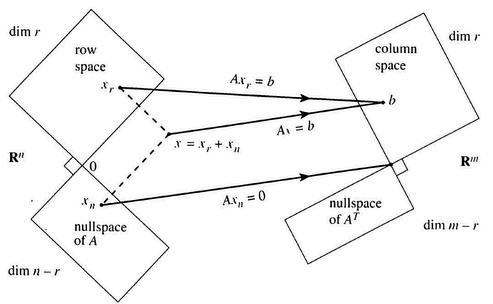
\includegraphics[width=0.7\linewidth]{images/four_spaces.png}

The rowspace of $A$ can be visualized using the line-intersection view of matrix-equations: it contains all the points that lie in the intersection of all the lines that make up the matrix. The columspace of A can be visulaized using the vector-image of A: it contains all the points that are spanned by A. 
Notice how we included the previous theorem: any combination $x$ of a particular sollution $x_r$ and any vector in the nullspace $x_n$ is also a solution.


\subsection{Spaces and eigenthingies}

\begin{definition}
Let $W$ be a space. Then $V \subseteq W$ is a subspace, if: 
    \begin{itemize}
        \item $\forall v_1, v_2 \in V: v_1 + v_2 \in W$
        \item $\forall v \in V: \forall r \in R: rv \in V$
    \end{itemize}
\end{definition}


\begin{definition}
    $B$ is linearly independent if $\forall b \in B: b \neq \sum r_n b_n$, with $b_n \in B/b$. 
\end{definition}

\begin{theorem}
  A better definition could be stated as such: $B$ is linearly independent, if the only solution to $Bx = 0$ is the zero-vector.
\end{theorem}

\begin{proof}
    \subprf{}{$( Bx = 0 \leftrightarrow \forall x_n = 0 ) \leftrightarrow (\forall b \in B: b \neq \sum r_n b_n, b_n \in B/b)$}{
        todo.
    }
\end{proof}

\begin{definition}
    Let $V$ be a subspace. $B \subseteq V$ is a basis for $V$ if $B$ is linearly independent and $\forall v \in V: v = \sum r_n b_n$, with $b_n \in B$
\end{definition}


\subsection{Rank nullity Theorem}

\begin{proof}
    $$ \nullspace{A} = \left{0\right} \then \det{A} \neq 0 $$
\end{proof}

\begin{proof}
    Let $A: X \to Y$. Then:
    $$ \nullspace{A} = \left{0\right} \then \collspace{A} = Y $$
\end{proof}

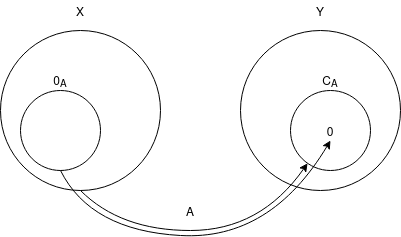
\includegraphics[width=0.4\linewidth]{images/A_from_X_to_Y.png}

\begin{proof}
    Rank nullity: this is a fundamental theorem of linear algebra.
    Let $A$ be of dimension $r \times c$ and full rank.
    Then: 
    $$ r_A + n_A = c $$
\end{proof}


\begin{proof}
    $$ r_A = dim_{C_A} = dim_{R_A} $$
\end{proof}

\begin{proof}
    $$ A:basis_{C_A} \then r_A = n $$
\end{proof}


\subsection{Inverses and determinant}

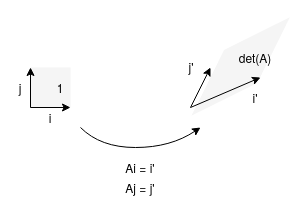
\includegraphics[width=0.4\linewidth]{images/determinant.png}

If $A$ has dimensions $n \times n$, then the inverse $A^{-1}$ such that
$$ A A^{-1} = A^{-1} A = I $$
exists iff $det_A \neq 0$.

\paragraph{Nonsqare} matrices do not have an inverse, but they might have a right- or left-inverse.
Consider $C = A A^T$. This is a square matrix, so it might have an inverse:
$$ A A^T (A A^T)^{-1} = I $$
Calling $A^T (A A^T)^{-1} = A^{RI}$ the right inverse:
$$ A A^{RI} = I $$
For $C^{-1}$ to exist, we require $C$ to be full-rank, which means that $A$ must be full row rank. This  requires $r \leq c$, in other words, $A$ being a broad matrix.

\begin{proof}
If $A^{RI}$ exists, then $A^{LI}$ does not
\end{proof}

\begin{proof}
    $A^{RI}$ is not unique.
    Let $A$ be of dimension $r \times c$ and full rank, with $r < c$. By rank nullity we have
    $$ n_A = c - r > 0 $$
    That is, the nullspace is nonempty. Thus $\thereis x : Ax = 0$
    Now try $B' = B + x$
    We get 
    $$ AB' = AB + Ax = I + 0$$
\end{proof}


\subsection{Change of basis}\label{changeOfBasis}

Let $V$ be a vector space. Let $0$ be the canonical basis for that vector space. Let $A = \{\vec{a}_1, ..., \vec{a}_N \}$ and $B = \{\vec{b}_1, ..., \vec{b}_N\}$ be two other basis for that vectorspace. Let $\mtrx{A}$ be the matrix $[\vec{a}_1  ...  \vec{a}_N]$ and $\mtrx{B} = [\vec{b}_1 ... \vec{b}_N]$

Every vector $\vec{v}$ can be expressed as a linear sum of the basisvectors in $A$, that is $\vec{v} = \sum_n \alpha_n \vec{a}_n$. That same thing in matrix notation: $\vec{v} = \mtrx{A}(\vec{v})_A$, where $(\vec{v})_A$ is the coordinates $\alpha$ of $\vec{v}$ with respect to the basis $A$. Correspondingly, for $B$ we have $\vec{v} = \sum_n \beta_n \vec{b}_n = \mtrx{B}(\vec{v})_B$.

Note that within $A$ and $B$, we express the basevectors with respect to the canonical basis $0$, that is, we should really write $\mtrx{A} = [(\vec{a}_1)_0  ...  (\vec{a}_N)_0]$. Note also that $[(\vec{a}_1)_A  ...  (\vec{a}_N)_A] = \mtrx{I}$, the identity matrix. 

We can use this to obtain a simple formula for the change of basis. 
$$ \vec{v} = \mtrx{A} (\vec{v})_A $$
$$ \vec{v} = \mtrx{B} (\vec{v})_B $$
$$ (\vec{v})_B = \mtrx{B}^{-1} \mtrx{A} (\vec{v})_A $$

But inverses are notoriously hard to calculate. Fortunately, there is another approach. Call $\mtrx{T}_{BA} = [(\vec{a}_1)_B ... (\vec{a}_N)_B]$ the \emph{transition matrix}. We can prove that $\mtrx{B}^{-1} \mtrx{A} = \mtrx{T}_{BA}$:

\begin{equation}
\begin{aligned}
\mtrx{B}^{-1} \mtrx{A} (\vec{v})_A &= \mtrx{T}_{BA}  (\vec{v})_A \\
                                   &= \sum_n (v_n)_A (\vec{a}_n)_B \\
                                   &= \sum_n (v_n)_A \mtrx{B}^{-1} \mtrx{A} (\vec{a}_n)_A \\
                                   &= \mtrx{B}^{-1} \mtrx{A} \sum_n (v_n)_A (\vec{a}_n)_A \\
                                   &= \mtrx{B}^{-1} \mtrx{A} \text{  } \mtrx{I} (\vec{v})_A \\
                    (\vec{v})_A &=  (\vec{v})_A         
\end{aligned}
\end{equation}

Using $\mtrx{T}_{BA} = \mtrx{B}^{-1}\mtrx{A}$, a lot of statements are trivial to prove:
\begin{itemize}
    \item $\mtrx{T}_{BA} = \mtrx{T}_{AB}^{-1}$
    \item $\mtrx{T}_{CA} = \mtrx{T}_{CB} \mtrx{T}_{BA}$
\end{itemize}


\subsection{Linear transformations}

\begin{definition}
Let $U$ and $V$ be two vector spaces and $f:U \to V$. Then $f$ is a \emph{linear transform} if
\begin{itemize}
    \item $f$ preserves scalar multiplication: $f(\alpha \vec{u}) = \alpha f(\vec{u})$
    \item $f$ preserves vector addition: $f(\vec{u}_1 + \vec{u}_2) = f(\vec{u}_1) + f(\vec{u}_2)$
\end{itemize}
\end{definition}

There are a bunch of properties to linear transformations that can be useful to us. 

\begin{proof}[There is a unique linear transform from the basis of $U$ to any set of vectors in $V$ that we want.] In other words, any linear transform $f$ is completely deterimed by the matrix $[ f(\vec{b}_1) ... f(\vec{b}_N) ] = [\vec{v}_1 ... \vec{v}_N]$. That means if we dont know the transform, but we do know the results of the transform on a basis, then we can reconstruct the transform with certainty.  \\

    \subprf{Let $B = \{ \vec{b}_1, ..., \vec{b}_N \}$ be a basis for $U$. Let $\{ \vec{v}_1, ..., \vec{v}_N \}$ be any vectors in $V$ that we may chose. }
    { there is a unique function $f:U \to V$ such that $f(\vec{b}_i) = \vec{v}_i$ }{
    
        \subprf{Try $f(\vec{x}) = \mtrx{V} (\vec{x})_B$}
        {$f(\vec{b}_i) = \vec{v}_i$ and $f$ is a linear transform.}{
        
            \subprf{Part 1: }
            {$f(\vec{b}_i) = \vec{v}_i$}{
                
                $ f(\vec{b}_i) = \mtrx{V} (\vec{b}_i)_B = \mtrx{V} \vec{e}_i = \vec{v}_i $
                
            }
            
            \subprf{Part 2: }{$f$ is unique}{
                
                We could not have obtained any other form of $f$ than $f(\vec{x}) = \mtrx{V} (\vec{x})_B$. This is because for \emph{any} linear transform from $U \to V$ we have: 
                
                $ f(\vec{x}) = f(\mtrx{B}(\vec{x})_B) = f(\sum_n (x_n)_B \vec{b}_n) = \sum_n (x_n)_B f(\vec{b}_n)  $
                
                Using the result from part 1, this cannot be any other function than: 
                
                $ \sum_n (x_n)_B f(\vec{b}_n) = \sum_n (x_n)_B \vec{v}_n = \mtrx{V} (\vec{x})_B $ 
                
            }
            
            \subprf{Part 3: }
            {$f$ is a linear tansform}{
            
            }
        }
    }
\end{proof}

A whole bunch of other properties are now easily proved. Let $f$ and $g$ be linear transforms from $U$ to $V$. The following are also linear transforms: 
\begin{itemize}
    \item $\alpha f$
    \item $f + g$
    \item $f^{-1}$ ( if it exists )
    \item $fg$ ( here $g: V \to W$ )
\end{itemize}

Let $f: U \to V$ be a linear transform. Then the following are equivalent: 
\begin{itemize}
    \item If $f(\vec{u}) = \vec{0}$, then $\vec{u} = \vec{0}$
    \item $f$ is one-to-one
    \item $f$ maps linearly independent vectors to linearly independent vectors. 
\end{itemize}


Prove that a transform can be split up into mulitple transforms on the basis vectors. 
As an examle, consider the case of a rotation. A diagonal rotation can be reproduced by a rotation first around one, then around another axis. 


\paragraph{A linear transformation can also be a change of basis} when it is on a vectorspace and invertible.


\subsection{Systems of linear equations}
If there are more variables than equations, the system is underdetermined. If there are more eqations than variables, the system is overdetermined. A potentially solveable system is one where there are equally many variables as equations. But even then we must distinguish two cases. 

\subsubsection{Solving well determined systems}
There are two cases: a system is either consistent or inconsistent. The follwing statements are all equivalent, meaning that any one of them is related to any other one in an if-and-only-if way. 

\begin{itemize}
    \item the system is consistent
    \item the matrix is invertible
    \item the determinant is nonzero
    \item there is exactly one sollution
\end{itemize}

We proof a few of those equivalences just for the hell of it. 

\begin{proof} There is exactly one solution if and only if the determinant is nonzero. \\
    \subprf{}{$|A| = 0 \iff \thereis ! \vec{x} : A \vec{x} = \vec{b} $}{
    
    }
\end{proof}

On the other hand, in the inconsistent case, the follwing statements are equivalent:

\begin{itemize}
    \item the system is inconsistent
    \item the matrix is singular (aka. noninvertible)
    \item the determinant equals zero
    \item one (or more) row (or column) is lineraly dependent of the others
\end{itemize}

\subsubsection{Solving overdetermined systems: least squares}


\subsubsection{Solving underdetermined systems: geometric bodies}
I like to think of underdetermined systems as (linear) geometric bodies, written in their parameterized form. A line in $\reals^3$ is described by a $3 \times 1$ matrix (or rather, it's column space), a plane in $\reals^3$ by a $3 \times 2$ matrix. However, it is important to note one distinction: geometric objects don't need to go through the origin, a matrix system however does. A line that does not go through the origin needs a base vector, like so: 

$$\vec{x} = \begin{bmatrix} \vec{d} \end{bmatrix} \begin{bmatrix} \alpha \end{bmatrix} + \vec{b}$$ 

A plane that does not go through the origin also needs a base vector $\vec{b}$, like so: 

$$\vec{x} = \begin{bmatrix} \vec{p}_1 && \vec{p}_2 \end{bmatrix} \begin{bmatrix} \alpha  \\ \beta \end{bmatrix} + \vec{b}  $$



Here is a problem that bothered me for a while: a line needs one parameter, a plane two. An ellipsoid, too, needs two parameters. Are there any linear geometric objects in $\reals^3$ that require more than three parameters? The answer is: no. Here is the proof. 

\begin{proof}
    For any $3 \times 4$ matrix, there is a $3 \times 3$ matrix that has the same column space, that is, that describes the same geometrical body. \\
    
    \subprf{}{$\forall A(3 \times 4) \thereis A'(3 \times 3): \collspace{A} = \collspace{A'}$}{

        \subprf{Let $A_0(3 \times4)$.}{$\thereis A': \collspace{A_0} = \collspace{A'}$}{
        
            We know from \ref{proofBaseSizeEqualsSpaceDimension} that $\thereis \vec{a}_0 \in A_0: \vec{a}_0:ld$. So Try $A' = A_0/\vec{a_0}$.
            
            Indeed, now $A_0$ and $A'$ both form a base of the same space. So they must have the same column space. 
        }    

    }
\end{proof}

However, there are \emph{non}linear objects in $\reals^3$ that require more than three parameters! Many curves in 3d require many parameters. \emph{But} those curves don't form a vector-space, while lines and planes do (as long as they go through the origin). 


\subsubsection{Summary}
\begin{table}[ht]
\centering
\caption{Influence of rank on solutions}
\begin{tabular}{@{}llll@{}}
\toprule
                                                                                      & m \textless n                             & m = n & m \textgreater n                                 \\ \midrule
\rowcolor[HTML]{96FFFB} 
\cellcolor[HTML]{96FFFB}                                                              & n - m free variables                      &       &                                                  \\
\rowcolor[HTML]{96FFFB} 
\multirow{-2}{*}{\cellcolor[HTML]{96FFFB}r \textless m}                               & m – r conditions on $b \in \collspace{A}$ &       &                                                  \\
                                                                                      & 1 pivot per row                           &       &                                                  \\
                                                                                      & n – r = n – m free variables              &       &                                                  \\
\multirow{-3}{*}{\begin{tabular}[c]{@{}l@{}}r = m \\ (full row rank)\end{tabular}}    & 0 conditions on $b \in \collspace{A}$     &       & X                                                 \\
\rowcolor[HTML]{96FFFB} 
\cellcolor[HTML]{96FFFB}                                                              &                                           &       & m – r conditions on $b \in \collspace{A}$        \\
\rowcolor[HTML]{96FFFB} 
\multirow{-2}{*}{\cellcolor[HTML]{96FFFB}r \textless n}                               &                                           &       & n – r free variables                             \\
                                                                                      & X                                         &       & 1 pivot per column                               \\
                                                                                      &                                           &       & m – r = m – n conditions on $b \in \collspace{A}$ \\
\multirow{-3}{*}{\begin{tabular}[c]{@{}l@{}}r = n \\ (full column rank)\end{tabular}} &                                           &       & 0 free variables, thus $\nullspace{A} = \{0\}$     \\ \cmidrule(l){1-4} 
\end{tabular}
\end{table}


